\documentclass[border=4pt]{standalone}
\usepackage{fontspec}
\setmainfont{texgyretermes-regular.otf}[BoldFont=texgyretermes-bold.otf,ItalicFont=texgyretermes-italic.otf]
\usepackage{tikz}
\usetikzlibrary{shapes.geometric,calc}
\begin{document}
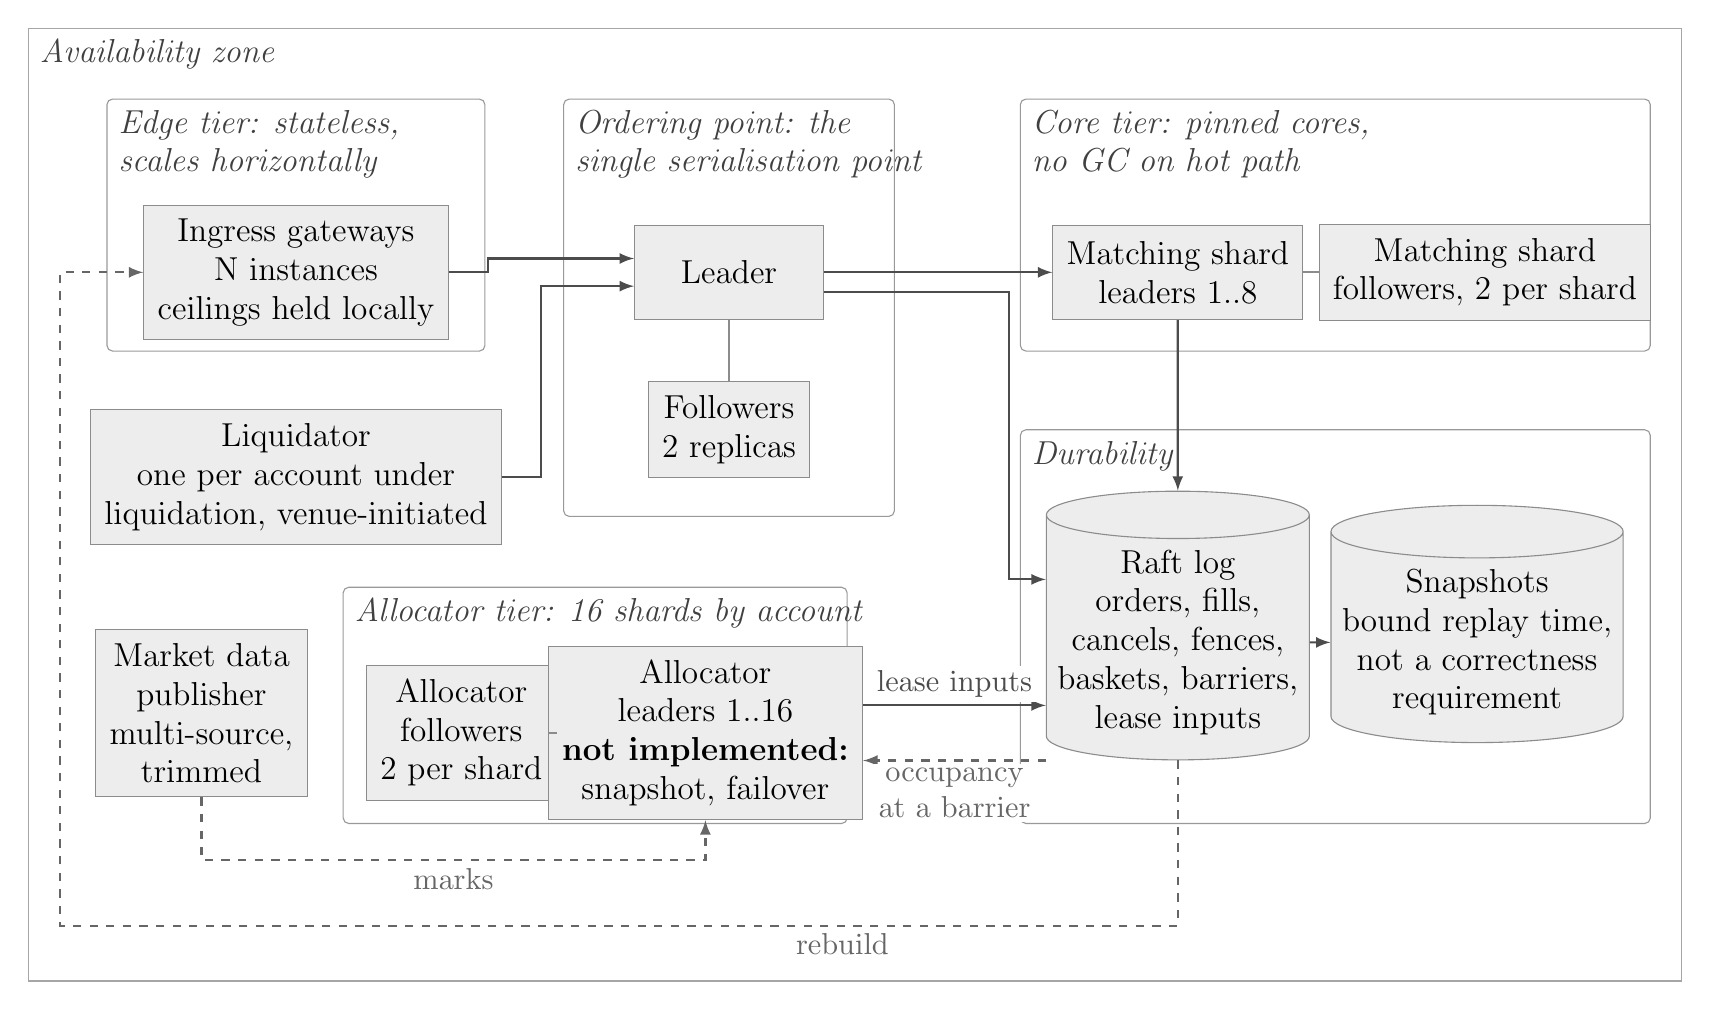
\begin{tikzpicture}[font=\fontsize{12}{14}\selectfont,
  box/.style={draw=black!45,fill=black!7,align=center,inner sep=5pt,minimum height=1.2cm},
  tier/.style={draw=black!40,rounded corners=2pt},
  title/.style={anchor=north west,align=left,inner sep=4pt,font=\fontsize{11.5}{13.5}\selectfont\itshape,text=black!75},
  db/.style={cylinder,shape border rotate=90,aspect=0.18,draw=black!45,fill=black!7,align=center,inner sep=4pt,minimum height=2.6cm,minimum width=3.0cm},
  flow/.style={-latex,black!70,thick},
  async/.style={-latex,black!60,thick,dashed},
  lab/.style={font=\fontsize{11}{13}\selectfont,fill=white,inner sep=1.5pt,align=center}]

% Edge tier and liquidator
\draw[tier] (0,6.0) rectangle (4.8,9.2); \node[title] at (0,9.2) {Edge tier: stateless,\\scales horizontally};
\node[box] (gw) at (2.4,7.0) {Ingress gateways\\N instances\\ceilings held locally};
\node[box] (lq) at (2.4,4.4) {Liquidator\\one per account under\\liquidation, venue-initiated};
% Ordering point
\draw[tier] (5.8,3.9) rectangle (10.0,9.2); \node[title] at (5.8,9.2) {Ordering point: the\\single serialisation point};
\node[box,minimum width=2.4cm] (opl) at (7.9,7.0) {Leader};
\node[box] (opf) at (7.9,5.0) {Followers\\2 replicas};
\draw[black!45,thick] (opl) -- (opf);
% Core tier
\draw[tier] (11.6,6.0) rectangle (19.6,9.2); \node[title] at (11.6,9.2) {Core tier: pinned cores,\\no GC on hot path};
\node[box] (ms) at (13.6,7.0) {Matching shard\\leaders 1..8};
\node[box] (msr) at (17.5,7.0) {Matching shard\\followers, 2 per shard};
\draw[black!45,thick] (ms) -- (msr);
% Durability
\draw[tier] (11.6,0.0) rectangle (19.6,5.0); \node[title] at (11.6,5.0) {Durability};
\node[db] (rl) at (13.6,2.3) {Raft log\\orders, fills,\\cancels, fences,\\baskets, barriers,\\lease inputs};
\node[db] (sn) at (17.4,2.3) {Snapshots\\bound replay time,\\not a correctness\\requirement};
% Allocator tier
\draw[tier] (3.0,0.0) rectangle (9.4,3.0); \node[title] at (3.0,3.0) {Allocator tier: 16 shards by account};
\node[box] (alr) at (4.5,1.15) {Allocator\\followers\\2 per shard};
\node[box] (al) at (7.6,1.15) {Allocator\\leaders 1..16\\\textbf{not implemented:}\\snapshot, failover};
\draw[black!45,thick] (alr) -- (al);
% Market data
\node[box] (md) at (1.2,1.4) {Market data\\publisher\\multi-source,\\trimmed};

\coordinate (a1) at ($(al.east)+(0,0.35)$); \coordinate (a2) at ($(al.east)+(0,-0.35)$); \coordinate (r0) at ($(rl.west)+(0,0.8)$);
% order path and log writes
\draw[flow] (gw.east) -- ++(0.5,0) |- ([yshift=5pt]opl.west);
\draw[flow] (lq.east) -- ++(0.5,0) |- ([yshift=-5pt]opl.west);
\draw[flow] (opl.east) -- ++(0.6,0) |- (ms.west);
\draw[flow] ([yshift=-7pt]opl.east) -- ++(2.35,0) |- (r0);
\draw[flow] (ms.south) -- (rl.north);
\draw[flow] (a1) -- node[lab,above=1pt]{lease inputs} (a1 -| rl.west);
\draw[flow] (rl.east) -- (sn.west);
% asynchronous
\draw[async] (a2 -| rl.west) -- node[lab,below=1pt]{occupancy\\at a barrier} (a2);
\draw[async] (md.south) -- ++(0,-0.8) -| node[lab,pos=0.25,below=1pt]{marks} (al.south);
\draw[async] (rl.south) -- ++(0,-2.1) -| node[lab,pos=0.15,below=1pt]{rebuild} (-0.6,7.0) -- (gw.west);

% availability zone
\draw[black!35] (-1.0,-2.0) rectangle (20.0,10.1); \node[title] at (-1.0,10.1) {Availability zone};
\end{tikzpicture}
\end{document}
